\chapter{Theoretical and Experimental Overview} \label{ch::theory_exp}
\ifpdf
\graphicspath{{Chapters/Theory/Figs/Raster/}{Chapters/Theory/Figs/PDF/}{Chapters/Theory/Figs/}}
\else \graphicspath{{Chapters/Theory/Figs/Vector/}{Chapters/Theory/Figs/}}
\fi

\section{The Structure of the Nucleon}

\subsection{Deep Inelastic Scattering}
To understand the structure of the nucleon it is useful to introduce the first
process which described the nucleon as having a sub-structure.  This process is
the Deep Inelastic Scattering (DIS) process where a lepton impinges on a
nucleon.  This is denoted as

\begin{equation}
\ell(l) + N(P) \rightarrow \ell(l') + X,
\end{equation}
\noindent
where $\ell$ denotes a lepton, $N$ denotes a nucleon, $X$ represents all
products not detected and $l$, $l'$ and $P$ are four momentum for their
respective leptons or nucleon.  The leading order Feynman diagram for this
reaction is show in Fig.~\ref{fig::DIS_LO}.

%\begin{figure}[h!t]
%  \centering
%  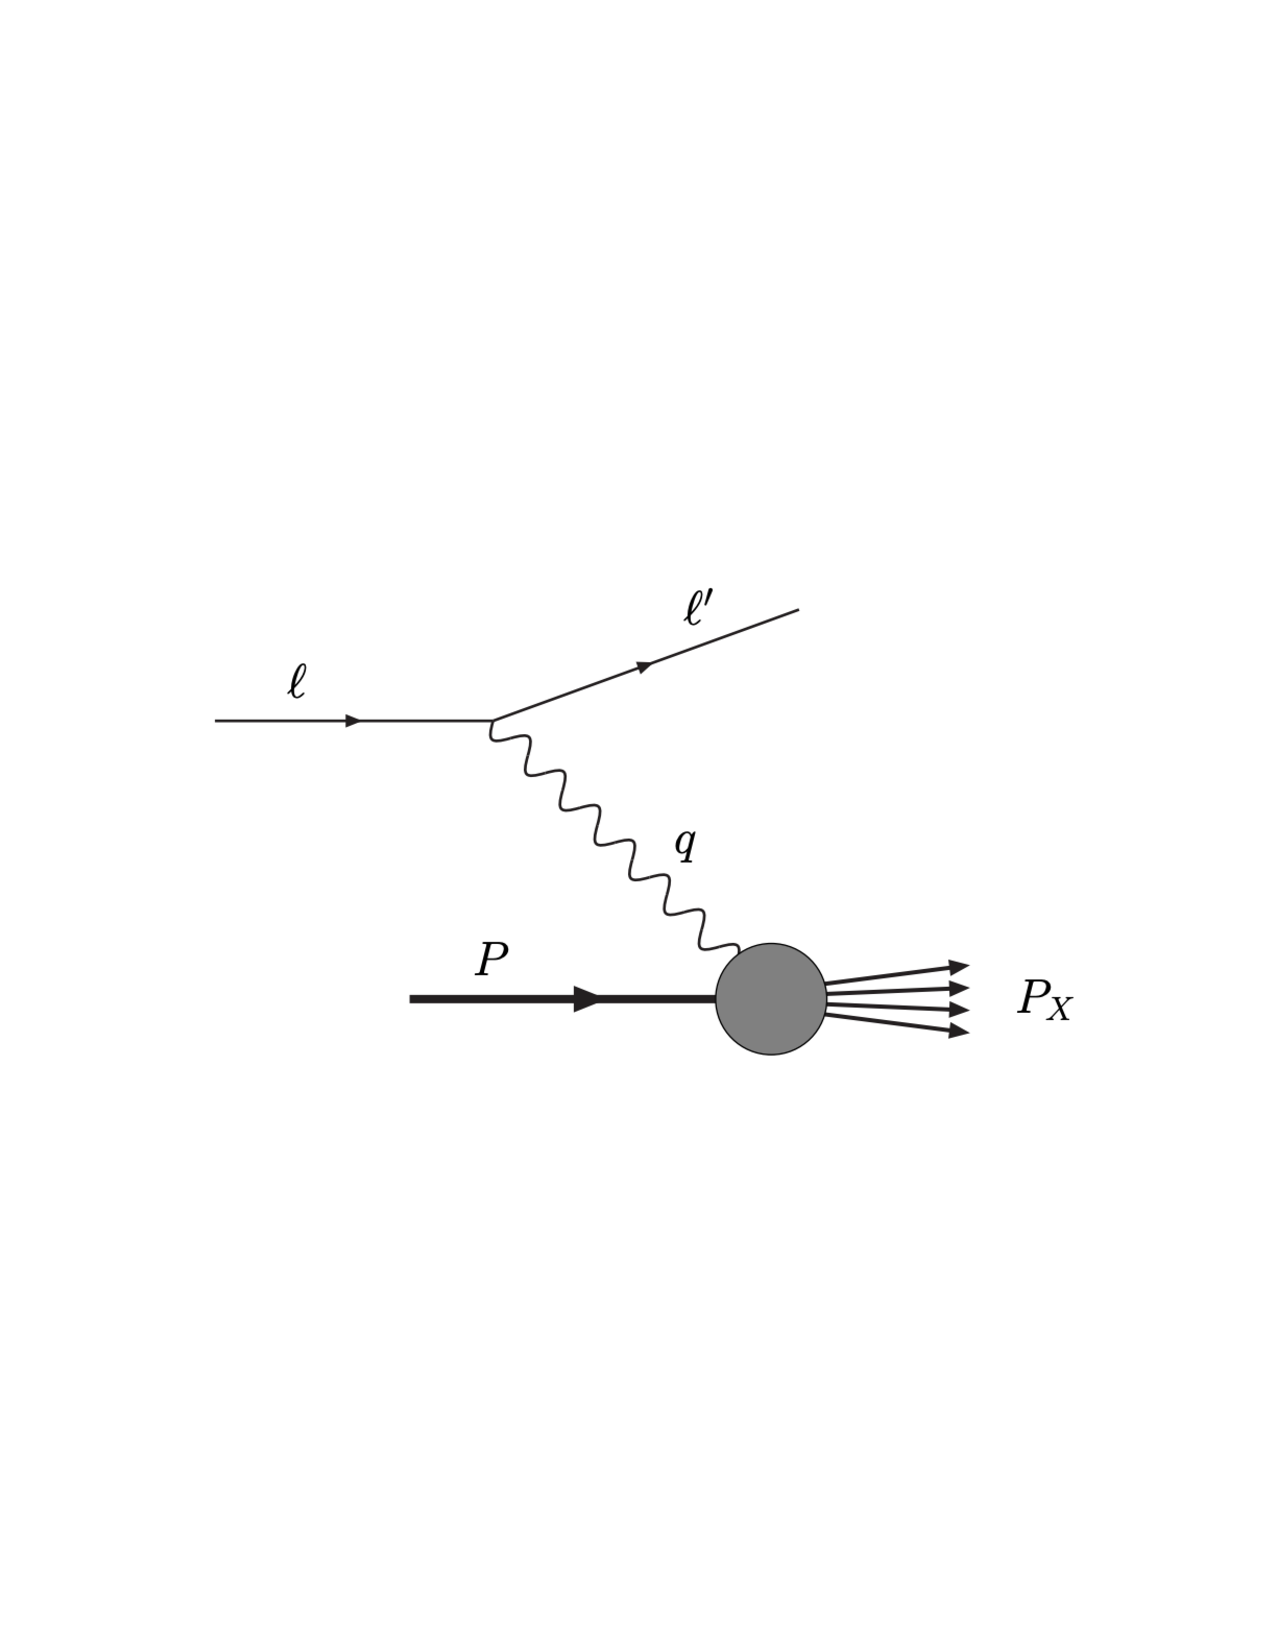
\includegraphics[width=0.6\textwidth]{DIS_LO}
%  \caption{The lead order Feynman diagram for deep inelastic scattering}
%  \label{fig::DIS_LO}
%\end{figure}

DIS is traditionally studied with a high energy lepton beam and a fixed nuclear
target.  The initial state kinematics are described by

\begin{equation}
 s = (l+P)^2 \quad \mathrm{or} E,
\end{equation}
\noindent
where $s$ is the center of mass energy and $E$ is the energy of the lepton beam.
The final state kinematics are described by

\begin{equation}

\end{equation}
